\chapter{Event generation, simulation and reconstruction}\label{ch:gensimreco}

\noindent The process of analyzing the data recorded by the CMS experiment involves several stages where the data are processed in order to interpret the information provided by all the detection systems; in those stages the particles produced after the \pp collision are identified by reconstructing their trajectories and measuring their features. In addition, the SM provides a set of predictions that have to be compared with the experimental results; however, in most of the cases, theoretical predictions are not directly comparable to experimental results due to the diverse source of uncertainties introduced by the experimental setup and theoretical approximations among others.\\

\noindent The strategy to face these conditions consist in using statistical methods implemented in computational algorithms to produce numerical results that can be contrasted with the experimental results. These computational algorithms are commonly known as Monte Carlo (MC) methods and, in the case of particle physics, they are designed to apply the SM rules and produce predictions about the physical observables measured in the experiments. Since particle physics is governed by quantum mechanics principles, predictions are not allowed for single events; therefore, a high number of events are ``generated'' and predictions are produced in the form of statistical distributions for the observables. Effects of the detector presence are included in the predictions by introducing simulations of the detector itself.\\     

\noindent This chapter presents a description of the event generation strategy and the tools used to perform the detector simulation and physics objects reconstruction. A comprehensive review on event generators for LHC physics can be found in reference \cite{gen} on which this chapter is based.  

\section{Event generation}

\begin{figure}[!h]
  \centering
  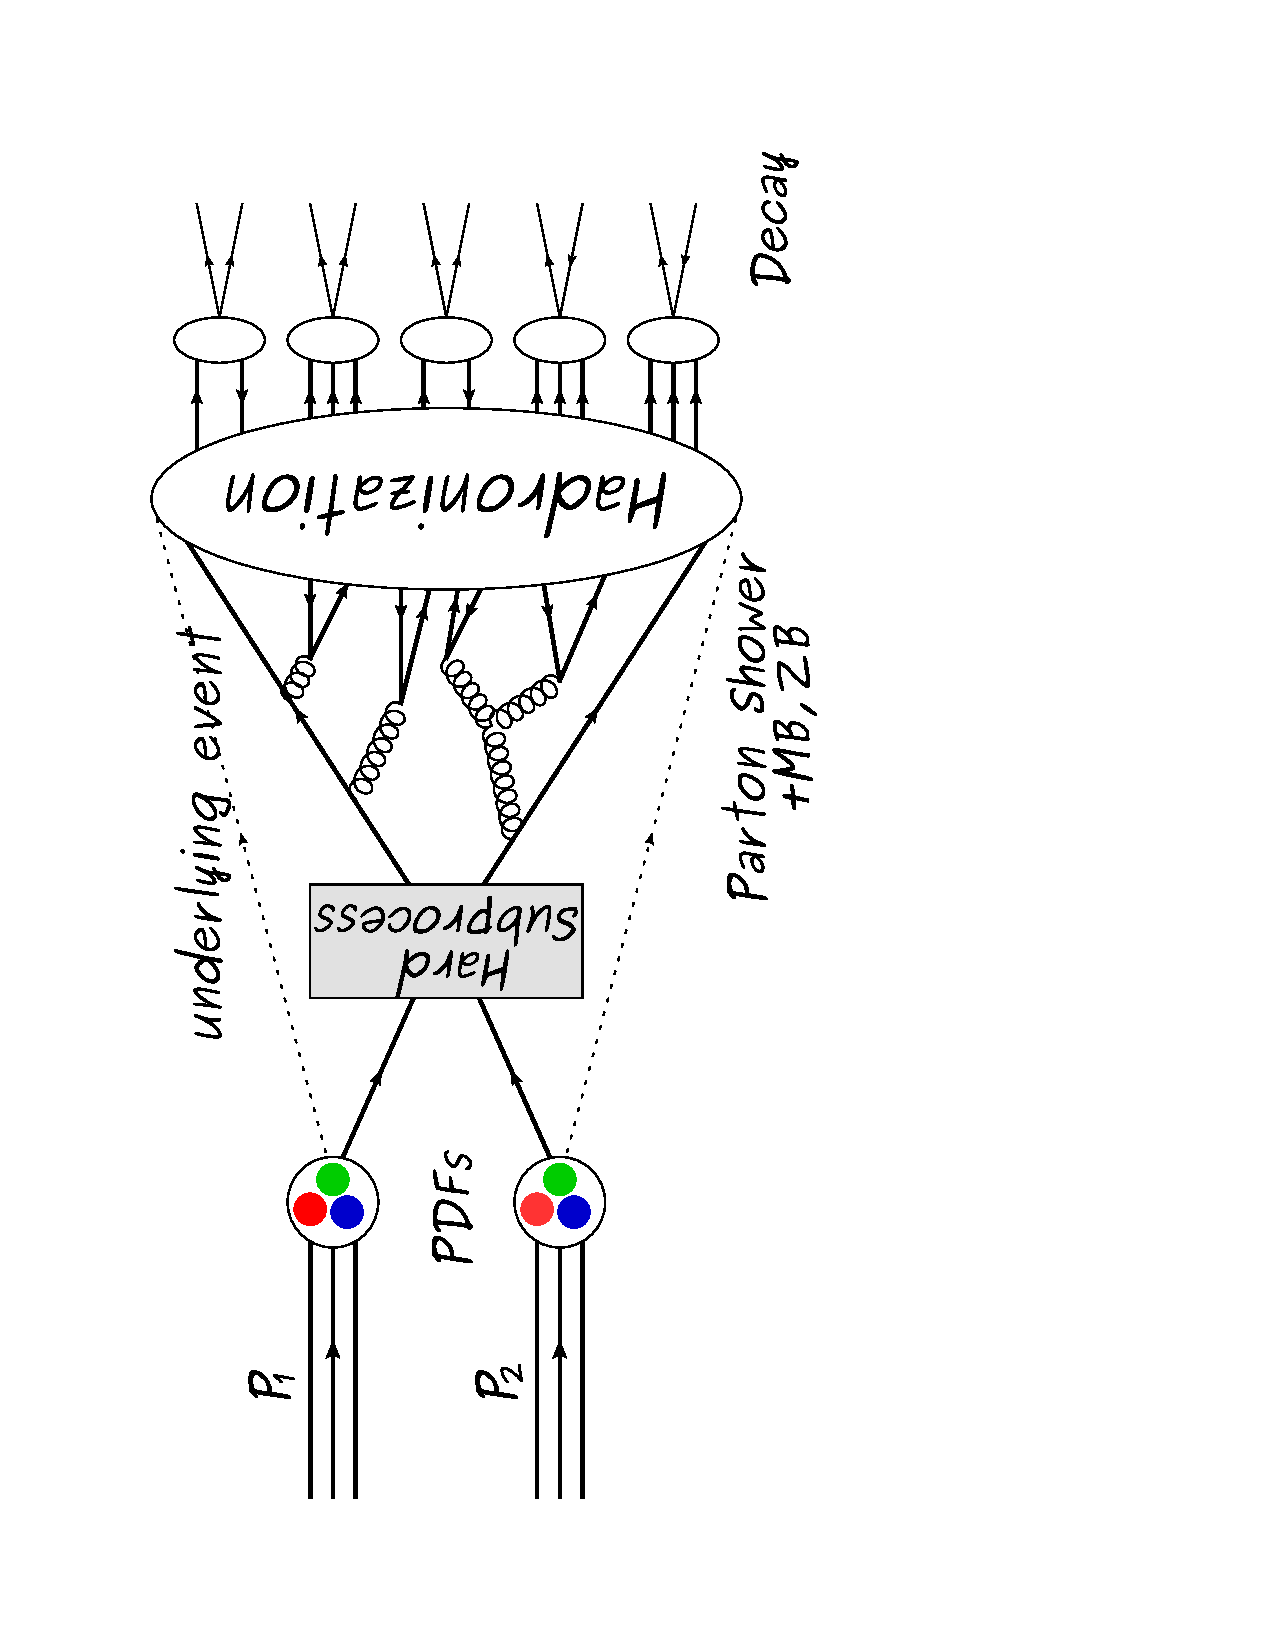
\includegraphics[scale=0.6,angle=-90]{gen}
  \caption[Event generation process.]{Event generation process. In the first step, the PDF of the colliding particles is considered so the specific interaction is described. The actual interaction is generated in the hard subprocess; the cross section of the process is calculated from the matrix element connecting the initial and final states. The parton shower describes the evolution of the partons from the hard subprocess according to the DGLAP equations. At this step the underlying event and PU effects are included in the generation. The resulting partons from the parton shower are recombined to form hadrons in the hadronization step; most of them are unstable, therefore, their decays are also generated in agreement to the known branching ratios. Modified from reference\cite{gen_scheme}.}\label{fig:gen}
\end{figure}

\noindent The event generation is intended to create events that mimic the behavior of actual events produced in the collisions; the obey a sequence of steps from the particles collision hard process to the decay process into the final state particles. Figure \ref{fig:gen} shows an schematic view of the event generation process; the fact that the full process can be treated as several independent steps is based on the QCD factorization theorem.\\     

\noindent Generation starts by taking into account the PDFs of the incoming particles. Event generators offer the option to chose from several PDF sets depending on the particular process under simulation\footnote{Tool in Reference \cite{pdfplot} allows to plot different PDF sets under customizable conditions.}; in the following \pp collisions will be considered. The \textit{hard subprocess} describes the actual interaction between partons from the incoming protons; it is represented by the matrix element connecting the initial and final states of the interaction. Normally, the matrix element can be written as a sum over Feynman diagrams and consider interferences between terms in the summation. During the generation of the hard subprocess, the production cross section is calculated.\\ 

\noindent The order to which the cross section is calculated depends on the order of the Feynman diagrams involved in the calculation; therefore, radiative corrections are included by considering a higher order Feynman diagrams where QCD radiation dominates. Currently, cross sections calculated to LO do not offer a satisfactory description of the processes, \ie, the results are only reliable for the shape of distributions; therefore, NLO calculations have to be performed with the implication that the computing time needed is highly increased.\\       

\noindent The final parton content of the hard subprocess is subjected to the \textit{parton shower} which generates the gluon radiation. Parton shower evolves the partons; \ie, glouns split into quark-antiquark pairs and quarks of enough energy radiate gluons giving rise to further parton multiplication, following the DGLAP (Dokshitzer-Gribov-Lipatov-Altarelli-Parisi) equations. Showering continues until the energy scale is low enough to reach the non-perturbative limit.\\   

\noindent In the simulation of LHC processes that involve $b$ quarks like the single top quark or Higgs associated production, it is needed to consider that the $b$ quark is heavier that the proton; in this sense, the QCD interaction description is made in two different schemes \cite{schemes}

\begin{itemize}

\item four-flavor (4F) scheme. $b$ quarks appears only in the final state because they are heavier than the proton and therefore they can be produced only from the splitting of a gluon into pairs or singly in association with a $t$ quark in high energy-scale interactions. During the simulation, the $b$-PDFs are set to zero because it cannot be part of the proton. Calculation in this scheme are more complicated due to the presence of the second $b$ quark but the full kinematics is considered already at LO and therefore the accuracy of the description is better.   

\item five-flavor (5F) scheme. $b$ quarks are considered massless, therefore they can appear in both initial and final states since it can now be part of the proton; thus, during the simulation $b$-PDFs are not set to zero. In this scheme, calculations are simpler that in the 4F scheme and possible logarithmic divergences are absorbed by the PDFs through the DGLAP evolution.   
\end{itemize}

\noindent In this thesis, the \tHq events are generated using the 4F scheme in order to reduce uncertainties, while the \tHW events are generated using the 5F scheme to eliminate LO interference with the \ttH process\cite{demartin}.\\    

\noindent Partons involved in the \pp collision are the focus of the simulation, however, the rest of the partons inside the incoming protons are also affected because the remnants are colored objects; also, multiple parton interactions can occurs. The hadronization of the remnants and multiple parton interactions are known as ``underlying event'' and it has to be included in the simulation. In addition, multiple \pp collisions in the same bunch crossing (pile-up mentioned in \ref{sec:lhc}) occurs, actually in two forms

\begin{itemize}
\item \textit{in-time PU} which refers to multiple \pp collision in the bunch crossing but that are not considered as primary vertices. 
\item \textit{Out-of-time PU} which refers to overlapping \pp collisions from consecutive bunch crossings; this can occurs due to the time-delays in the detection systems where information from one bunch crossing is assigned to the next or previous one. 
\end{itemize}

\noindent While the underlying event effects are included in generation using generator-specific tools, PU effects are added to the generation by overlying Minimum-bias (MB) and Zero-bias (ZB) events to the generated events. MB events are inelastic events selected by using a loose (minimum bias) trigger with as little bias as possible, therefore accepting a large fraction of the overall inelastic event; ZB events correspond to random events recorded by the detector when collisions are likely. MB model in-time PU and ZB model out-of-time PU.\\ 

\noindent The next step in the generation process is called ``hadronization''. Since particles with a net color charge are not allowed to exits isolated, they have recombine to form bound states. This is precisely the process by which the partons resulting from the parton shower arrange themselves as color singlets to form hadrons. At this step, the energy-scale is low and the strong coupling constant is large, therefore hadronization process is non-perturbative and phenomenological model are used to describe the parton's evolution. Most of the baryons and mesons produced in the hadronization are unstable and hence they will decay in the detector.\\

\noindent The last step in the generation process corresponds to the decay of the unstable particles generated during hadronization; it is also simulated in the hadronization step, based on the known branching ratios. 

\section{Monte Carlo Event Generators.}

\noindent The event generation described in the previous section has been implemented in several software packages for which a brief description is given.     

\begin{itemize}

\item \textbf{PYTHIA 8}. It is a program designed to perform the generation of high energy physics events which describe the collisions between particles such as electrons, protons. Several theories and models are implemented in it, in order to describe physical aspects like hard and soft interaction, parton distributions, initial and final-state parton showers, multiple parton interactions, beam remnants, hadronization\footnote{based in the Lund string model\cite{lund}} and particle decay. Thanks to extensive testing, several optimized parametrizations known as ``tunnings'' have been defined in order to improve the description of actual collisions to a high degree of precision; for analysis at $\sqrt{s}=13$ TeV, the underline event CUETP8M1 tune is employed \cite{tune}.  The calculation of the matrix element is performed at LO which is not enough for the current required level of precision; therefore, pythia is often used for parton shower, hadronization, decays, while other event generators are used to generate the matrix element at NLO.
\item \textbf{MadGraph5\_aMC@NLO}. MadGraph is a matrix element generator which calculates the amplitudes for all contributing Feynman diagrams of a given process but does not provide a parton shower while MC@NLO incorporate NLO QCD matrix elements consistently into a parton shower framework; thus, MadGraph5\_aMC@NLO, as a merger of the two event generators MadGraph5 and aMC@NLO, is an event generator capable to calculate tree-level and NLO cross sections and perform the matching of those with the parton shower. It is one of the most frequently used matrix element generators; however, it has as particular feature the presence of negative event weights which reduce the number of events used to reproduce the the properties of the objects generated\cite{madgraph}.\\
\item \textbf{POWHEG}. It is an NLO matrix element generator where the hardest emission of color charged particles is generated in such a way that the negative event weights issue of MadGraph5\_aMC@NLO is overcome; however, the method requires an interface with  $p_T$-ordered parton shower or a parton shower generator where this highest emission can be vetoed in order to avoid double counting of this highest-energetic emission. PYTHIA is a commonly matched to POWHEG event generator\cite{powheg}.
\end{itemize}

\noindent Events resulting from the whole generation process are known as MC events. 

\section{CMS detector simulation.}

\noindent After generation, MC events contain the physics of the collisions but they are not ready to be compared to the events recorded by the experiment since these recorded events correspond to the response of the detection systems to the interaction with the particles traversing them. The simulation of the CMS detector have to be applied on top of the event generation; it is simulated with Geant4, a MC toolkit for the simulation of particles passing though matter which is also able to simulates the electronic signals that would be measured by all detectors inside CMS.\\   

\noindent The simulation takes the generated particles contained in the MC events as input, makes them to pass through the simulated geometry, and models physics processes that particles experience during their passage through matter. The full set of results from particle-matter interactions correspond to the simulated hit which contains information about the energy loss, momentum, position. Particles of the input event are called ``primary'', while the particles originating from GEANT4-modeled interactions of a primary particle with matter are called a ``secondary''.  Simulated hits are the input of subsequent modules that emulate the response of the detector readout system and triggers. The output from the emulated detection systems and triggers is known as digitization \cite{geant,geant2}.\\

\noindent The modeling of the CMS detector corresponds to the accurate modeling of the interaction among particles, the detector material and the magnetic field. This simulation procedure includes the following standard steps
\begin{itemize}
\item Modeling of the Interaction Region.
\item Modeling of the particle passage through the hierarchy of volumes that compose CMS detector and of the accompanying physics processes.
\item Modeling of the effect of multiple interactions per beam crossing and/or the effect of events overlay ( Pile-Up simulation).
\item Modeling of the detector's electronics response, signal shape, noise, calibration constants (digitization). 
\end{itemize}

\noindent In addition to the full simulation, \ie a detailed detector simulation, a faster simulations (FastSim) have been developed, that may be used where much larger statistics are required. In FastSim, detector material effects are parametrized and included in the hits; those hits are used as input of the same higher-level algorithms\footnote{track fitting, calorimeter clustering, b tagging, electron identification, jet reconstruction and calibration, trigger algorithms which will be considered in the next sections} used to analyze the recorded events. In this way, comparisons between fast and full simulations can be performed\cite{fastsim}.\\

\noindent After the full detector simulation, the output events can be directly compared with events actually recorded in the CMS detector. The collection of MC events that reproduce the expected physics for a given process are known as MC samples.

\section{Event reconstruction.}

\noindent In contrast to MC samples for which all the particles' information is available from it's identity to it's mass and energy, recorded events contain the electronic signals, provided by the CMS detection systems, encoding the interaction of physical particles with the detector matter; these electronic signals have to be combined in order to identify these particle and measure its features \ie, particles have to be ``reconstructed'' using the signals provided by the detection systems. The CMS experiment use the ``particle-flow event reconstruction algorithm (PF)'' to do reconstruction of particles produced in \pp collisions. Next sections will present a basic description of the \textit{Elements} used by PF: tracker tracks, energy clusters and muon tracks.   

\subsection{Particle-Flow Algorithm.}

\noindent Each of the several subdetection systems of the CMS detector is dedicated to identify specific type of particles, \ie, photons and electrons are absorbed by the ECAL and their reconstruction is based on ECAL information; hadrons are reconstructed from clusters in the HCAL while muons are reconstructed from hits in the muon chambers. PF is designed to correlate signals from all the detector layers (tracks and energy clusters) in order to reconstruct and identify each final state particle and its properties. For instance, a charged hadron is identified by a geometrical connection, know as \textit{link} between one or more calorimeter clusters and a track in the tracker provided there are no hits in the muon system; combining several measurements allows a better determination of the energy and charge sign of the charged hadron.   

\subsubsection*{Charged-particle track reconstruction.}

\noindent The strategy used by PF in order to reconstruct tracks is called ``Iterative Tracking'' which occurs in four steps

\begin{itemize}
\item Seed generation where initial track candidates are found by looking for combination of hits in the pixel detector, strip tracker and muon chambers. In total ten iterations are performed, each one with a different seeding requirement. Seeds are used to estimate the trajectory parameters and uncertainties at the time of the full track reconstruction. Seeds are also considered track candidates.    
\item Track finding using a tracking software known as Combinatorial Track Finder (CTF)\cite{ctf}. The seed trajectories are extrapolated along the expected flight path of a charged particle, in agreement to the the trajectory parameters obtained in the first step, in an attempt to find additional hits that can be assigned to the track candidates. 
\item Track-fitting where the found tracks are passed as input to a module which provides the best estimate of the parameters of each trajectory.
\item Track selection where track candidates are submitted to a selection which discards those that fail a set of defined quality criteria.
\end{itemize}

\noindent Iterations differ in the seeding configuration and the final track selection as elaborated in references \cite{particle_flow, particle_flow2}. In the first iteration, high \pt tracks and tracks produced near to the interaction region are identified and those hits are masked thereby reducing the combinatorial complexity. Next iterations search for more complicated tracks, like low \pt tracks and tracks from b hadron decays, which tend to be displaced from the interaction region.

\subsubsection*{Calorimeter clustering.}

\noindent After traversing the CMS tracker system, electrons, photons and hadrons deposit their energy in the ECAL and HCAL cells. The PF clustering algorithm aims to provide a high detection efficiency even for low-energy particles and an efficient distinction between close energy deposits. The clustering runs independently in the ECAL barrel and endcaps, HCAL barrel and endcaps, and the two preshower layers, following two steps
\begin{itemize}
\item cells with an energy larger than a given seed threshold and larger than the energy of the neighboring cells are identified as cluster seeds. The neighbor cells are those that either share a side with the cluster seed candidate, or the eight closest cells including cells that only share a corner with the seed candidate.
\item cells with at least a corner in common with a cell already in the cluster seed and with an energy above a cell threshold are grouped into topological clusters.
\end{itemize}

\noindent Clusters formed in this way are known as \textit{particle-flow clusters}. With this clustering strategy it is possible detect and measure the energy and direction of photons and neutral hadrons as well as differentiate these neutral particles from the charged hadron energy deposits. In cases involving charged hadrons for which the track parameters are not determined accurately, for instance low-quality and high-pT tracks, clustering helps in the energy measurements. 

\subsubsection*{Electron track reconstruction.}

\noindent Although the charged-particle track reconstruction described above works for electrons, they lose a significant fraction of their energy via bremsstrahlung photon radiation before reaching the ECAL; thus, the reconstruction performance depends on the ability to measure also the radiated energy. The reconstruction strategy in this case requires information from the tracking system and from the ECAL. Bremsstrahlung photons are emmited at similar \etac values to that of the electron but at different values of \phic; therefore, the radiated energy can be recovered by grouping ECAL clusters in a \etac window over a range of \phic around the electron direction. The group is called ECAL supercluster.\\

\noindent Electron candidates from the the track-seeding and  ECAL superclustering are merged into a single collection which is submitted to a full electron tracking fit with a Gaussian-sum filter (GSF)\cite{gsf}. The electron track and its associated ECAL supercluster form a \textit{particle-flow electron}.

\subsubsection*{Muon track reconstruction.}

\noindent Given that the CMS detector is equipped with a muon detection system capable to identify and measure the momentum of the muons traversing it, the muon reconstruction is not specific to PF; therefore, three different muon types are defined





• standalone muon. Hits within each DT or CSC detector are clustered to form track segments,
used as seeds for the pattern recognition in the muon spectrometer, to gather all DT, CSC, and
RPC hits along the muon trajectory. The result of the final fitting is called a standalone-muon
track.
• global muon. Each standalone-muon track is matched to a track in the inner tracker (hereafter
referred to as an inner track) if the parameters of the two tracks propagated onto a common
surface are compatible. The hits from the inner track and from the standalone-muon track are
combined and fit to form a global-muon track. At large transverse momenta, pT \& 200 GeV,
the global-muon fit improves the momentum resolution with respect to the tracker-only fit.
• tracker muon. Each inner track with pT larger than 0.5 GeV and a total momentum p in excess
of 2.5 GeV is extrapolated to the muon system. If at least one muon segment matches the
extrapolated track, the inner track qualifies as a tracker muon track. The track-to-segment
matching is performed in a local (x, y) coordinate system defined in a plane transverse to

the beam axis, where x is the better measured coordinate. The extrapolated track and the
segment are matched either if the absolute value of the difference between their positions in
the x coordinate is smaller than 3 cm, or if the ratio of this distance to its uncertainty (pull)
is smaller than 4.
Global-muon reconstruction is designed to have high efficiency for muons penetrating through
more than one muon detector plane. It typically requires segments to be associated in at least two
muon detector planes. For momenta below about 10 GeV, this requirement fails more often because
of the larger multiple scattering in the steel of the return yoke. For these muons, the tracker muon
reconstruction is therefore more efficient, as it requires only one segment in the muon system [35].
Owing to the high efficiency of the inner track and muon segment reconstruction, about 99%
of the muons produced within the geometrical acceptance of the muon system are reconstructed
either as a global muon or a tracker muon and very often as both. Global muons and tracker muons
that share the same inner track are merged into a single candidate. Muons reconstructed only as
standalone-muon tracks have worse momentum resolution and a higher admixture of cosmic muons
than global and tracker muons.
Charged hadrons may be misreconstructed as muons e.g. if some of the hadron shower remnants
reach the muon system (punch-through). Different identification criteria can be applied to the muon
tracks in order to obtain the desired balance between identification efficiency and purity. In the
PF muon identification algorithm (section 4.2), muon energy deposits in ECAL, HCAL, and HO
are associated with the muon track and this information is used to improve the muon identification
performance.








\noindent Once individual particles are identified and reconstructed, they can be grouped into larger objects to form jets. The reconstruction of all the particles in an event is used to determine the presence of neutrinos represented by an imbalance in the transverse energy.



Single particles give rise to different elements in the detector, thus a linking of these elements is required in order to reconstruct a particle correctly. The linker algorithm links two elements together on a trial basis and only keeps elements linked, if their quality surpasses a certain threshold. The linker tries to extrapolate tracks starting from the outermost hit in the silicon detector to either, the first two PS layers, the ECAL in depth of a typical maximum of an electromagnetic shower or the HCAL at a depth of a typical hadron shower length. If the extrapolated track is in correspondence up to a certain link distance with a calorimeter cluster the two elements are linked together. When linking tracks to ECAL clusters the trajectory of the track is extrapolated along its tangent, looking for energy deposits by bremsstrahlung. Elements directly or indirectly linked with each other are known as blocks. The high granularity of the CMS detector causes most blocks to only contain one to three elements and therefore the object reconstruction is simplified. The linking algorithm, as well as the whole particle flow algorithm, was intensively validated and commissioned [96] as e. g. a broken link could lead to a reconstruction of a ghost particle and thus to an overestimation of the total energy of the collision. In the last reconstruction step, the found blocks in the detector are interpreted as candidates, as they are reconstructed as actual physical objects.




CMS requires an offline first-pass full reconstruction of express line and all
online streams in quasi-realtime, which produces new reconstructed objects
called RECO data.




 vertexing , jets reco, anti-kt algorithm, jet energy corrections, btagging, MET 





The Tier-0 offline reconstruction step processes all RAW events from the online system following
an adjustable set of priorities (the express-line, by definition has very high priority). This step
creates new higher-level physics objects such as tracks, vertices, and jets. These may improve or
extend the set produced in the HLT processing step. It must run with minimal delay compared
to the online in order to provide rapid feedback to the online operations, for example, identifying
detector or trigger problems which can then be rectified dynamically during the same LHC fill.
The offline reconstruction will normally perform the same reconstruction steps for each stream,
with the possible exception of specialised calibration streams. In this way we ensure that they
are all useful in principle for all analysis groups. We apply this same rule to later re-processings
of the data, 2-3 times per year we expect to bring all datasets into consistent status as to applied
calibrations and algorithms, as described below.





\section{ MVA methods, NN, BDT, boosting, overtraining, variable ranking  }
\section{statistical inference, likelihood parametrization}
\section{ nuisance parameters}
\section{exclusion limits }
\section{asymptotic limits }












